\documentclass{article}

\usepackage{graphicx}
\usepackage{tikz}
\usepackage{tikzsymbols}
\usetikzlibrary{calc,patterns,shapes.geometric}
\pagestyle{empty}
\usepackage[margin=0pt]{geometry}
\geometry{papersize={14in,12in}}

\def\centerarc[#1](#2)(#3:#4:#5){\draw[#1] ($(#2)+({#5*cos(#3)},{#5*sin(#3)})$) arc (#3:#4:#5);}

\begin{document}
	\begin{figure}
		\centering
		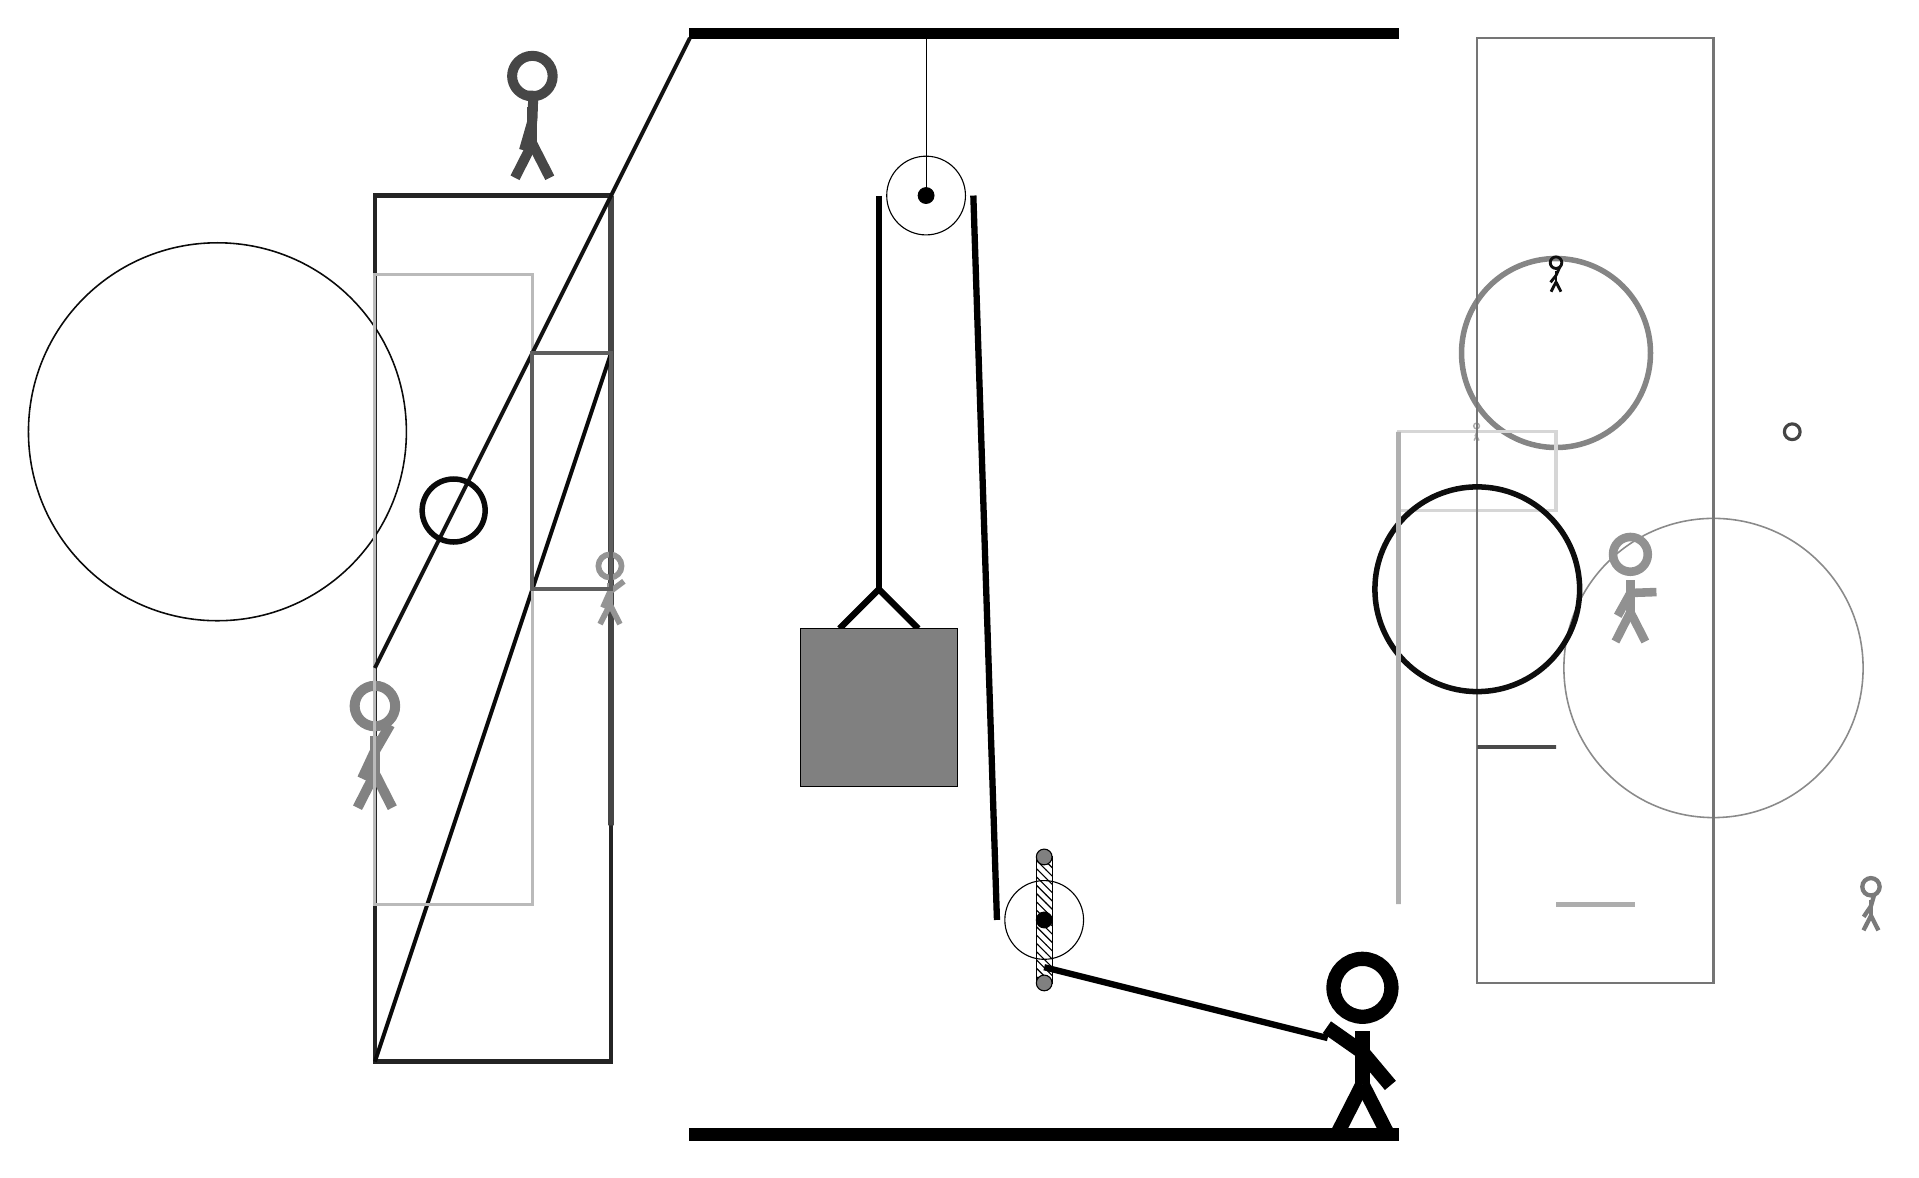
\begin{tikzpicture}
			%%%%% START %%%%%
			
			\draw[fill=black] (-2, 14) rectangle (7, 14.125);
			
			\draw[line width=0.6mm, color=black!86] (-3, 1) rectangle (-6, 12);
			
			\draw[line width=0.6mm, color=black!79] (-3, 11) rectangle (-3, 4);
			\node[line width=0.7mm, color=black!33] at (8, 9) {\Strichmaxerl[1][68][8]};
			\draw[line width=0.7mm, color=black!73] (-3, 4) rectangle (-3, 12);
			
			\draw [line width=0.7mm, color=black!48](9, 10) circle (1.2);
			\draw [line width=0.4mm, color=black!73](12, 9) circle (0.1);
			\draw [line width=0.2mm, color=black!46](11, 6) circle (1.9);
			\draw[line width=0.5mm, color=black!96](-6, 1) -- (-3, 10);
			\node[line width=0.4mm, color=black!94] at (9, 11) {\Strichmaxerl[2][51][66]};
			\draw[line width=0.4mm, color=black!16] (7, 9) rectangle (9, 8);
			\draw[line width=0.3mm, color=black!54] (8, 2) rectangle (11, 14);
			
			\draw [line width=0.2mm, color=black!96](-8, 9) circle (2.4);
			\node[line width=0.3mm, color=black!43] at (10, 7) {\Strichmaxerl[6][61][2]};
			
			\draw[line width=0.3mm, color=black!58] (7, 5) rectangle (7, 7);
			\node[line width=0.3mm, color=black!52] at (13, 3) {\Strichmaxerl[3][56][74]};
			\draw [line width=0.7mm, color=black!95](8, 7) circle (1.3);
			
			\node[line width=0.4mm, color=black!49] at (-6, 5) {\Strichmaxerl[7][65][60]};
			\draw[line width=0.4mm, color=black!27] (-4, 3) rectangle (-6, 11);
			\draw[line width=0.7mm, color=black!31] (7, 9) rectangle (7, 3);
			\draw[line width=0.5mm, color=black!93](-6, 6) -- (-2, 14);
			\node[line width=0.6mm, color=black!72] at (-4, 13) {\Strichmaxerl[7][74][88]};
			
			\node[line width=0.2mm, color=black!42] at (-3, 7) {\Strichmaxerl[4][66][37]};
			\draw[line width=0.5mm, color=black!63] (-4, 10) rectangle (-3, 7);
			\draw[line width=0.6mm, color=black!32] (9, 3) rectangle (10, 3);
			\draw[line width=0.5mm, color=black!71] (9, 5) rectangle (8, 5);
			
			\draw [line width=0.7mm, color=black!96](-5, 8) circle (0.4);
			
			\draw (1, 12) circle (0.5);
			\draw[fill=black] (1, 12) circle (0.1);
			\draw (1, 14) -- (1, 12);
			
			\draw[fill=white](2.5, 2.8) circle (0.5);
			\draw[fill=black] (2.5, 2.8) circle (0.1);
			\draw[pattern=north west lines, pattern color=black] (2.4, 3.6) rectangle (2.6, 2.0);
			\draw[fill=black!50] (2.5, 3.6) circle (0.1);
			\draw[fill=black!50] (2.5, 2.0) circle (0.1);
			
			\draw[line width=0.8mm] (-0.1, 6.5) -- (0.4, 7.0) -- (0.9, 6.5);
			\draw[fill=black!50] (-0.6, 6.5) rectangle (1.4, 4.5);
			
			\draw[line width=0.8mm] (0.4, 12) -- (0.4, 7.0);
			\centerarc[line width=0.8mm](1, 12)(0:180:0.6);
			\draw[line width=0.8mm](1.6, 12) -- (1.9, 2.8);
			\centerarc[line width=0.8mm](2.5, 2.8)(180:270:0.6);
			\draw[line width=0.8mm](2.5, 2.2) -- (6.1, 1.3);
			
			\node at (6.5, 1.2) {\Strichmaxerl[10][-35][-50]};
			
			\draw[fill=black] (-2, 0) rectangle (7, 0.15);
			
			%%%%% END %%%%%
		\end{tikzpicture}
	\end{figure}	
\end{document}